\documentclass[11pt,a4paper]{article}

\usepackage[utf8]{inputenc} 
\usepackage[T1]{fontenc} 
\usepackage{lmodern}
\usepackage[margin=2cm]{geometry}
\usepackage[german]{babel}
\usepackage{array}
\setlength{\parindent}{0pt}
\setlength{\parskip}{1ex plus 0.5ex minus 0.5ex}

\usepackage{amsmath} 
\usepackage{graphicx} 
\usepackage{booktabs}
\usepackage[colorlinks]{hyperref}
\usepackage{nicefrac}
\usepackage{gensymb}
\usepackage[usenames,dvipsnames,svgnames,table]{xcolor}
\usepackage{multirow}
\usepackage{tikz}
\usepackage[section]{placeins}
\usepackage{wrapfig}

\hbadness=99999

\newcommand{\refpy}[1]{Siehe Anhang: \textit{Rechnungen in Python} (\texttt{{\color{incolor}In [{\color{incolor}#1}]}})}
\newcommand\dif{\mathop{}\!\mathrm{d}}
\newcommand{\halftime}[4]{\begin{figure}[h]
\begin{minipage}{.#1\textwidth}#3\end{minipage}\begin{minipage}{.#2\textwidth}
\centering
#4\end{minipage}
\end{figure}}
\newcommand{\pard}[2]{\frac{\partial #1}{\partial #2}}
\newcommand{\bigp}[1]{\bigg(#1\bigg)}

\renewcommand{\vec}{\boldsymbol}

\usepackage{etoolbox}

\makeatletter
\patchcmd{\@classz}
  {\CT@row@color}
  {\oldCT@column@color}
  {}
  {}
\patchcmd{\@classz}
  {\CT@column@color}
  {\CT@row@color}
  {}
  {}
\patchcmd{\@classz}
  {\oldCT@column@color}
  {\CT@column@color}
  {}
  {}
\makeatother

\newcommand{\rpm}{\raisebox{.2ex}{$\scriptstyle\pm$}}

\begin{document}

{
\centering 
\large 
Physiklabor für Anf\"anger*innen \\
Ferienpraktikum im Sommersemester 2018 \\[4mm]
\textbf{\LARGE 
Versuch 17: Trägheitsmomente/Steinerscher Satz
} \\[3mm]
(durchgef\"uhrt am 17.09.2018 bei Adrian Hauber)\\
Gruppe 14: Andréz Gockel, Patrick M\"unnich\\ 
\today \\[10mm]
}
%\vspace{88pt}
\vfill
\tableofcontents
\vfill
%\vspace{22pt}
%\listoffigures
%\vspace{22pt}
%\listoftables
\pagebreak

\section{Ziel des Versuchs}

Dieser Versuch hat drei Teile. Im ersten Teil wird mit Hilfe von einer Herleitung das Trägheitsmoment mit der Periodendauer in Zusammenhang gebracht, hiermit wird der Satz von Steiner überprüft.  

In dem zweiten Teil wird dann der theoretisch berechnete Wert verglichen mit dem experimentell bestimmten Wert. 

In dem dritten Teil wird mit einem Drehpendel der Zusammenhang von der Schwingungsdauer und dem Abstand von einer Zusatzmasse zum Mittelpunkt untersucht.
\section{Teil 1 - Trägheitsmomente}
\subsection{Herleitung der Schwingungsgelichung}

Der unterschied von einem mathematischen Pendel und einem physikalischen Pendels ist, dass es sich beim Physikalischen nicht um eine punktförmige Masse handelt, sondern der Schwerpunkt von einem starren Körper zur Rechnung verwendet wird, wobei das Trägheitsmoment berücksichtigt werden muss. Mit der rücktreibenden Kraft $F_r = -mg\sin\varphi$ und dem Abstand vom Aufhängepunkt zu Schwerpunkt $d$ können wir das Drehmoment ausdrücken als:
$$\vec{M} = -\vec{F_r} \times \vec{d} = dm\vec{g}\sin(\varphi)$$
mit der Kleinwinkelnäherung: $\sin\varphi \approx \varphi$:
$$\vec{M} = dm\vec{g}\varphi$$
Dies wird gleichgesetzt mit:
$$\vec{M} = \vec{\dot L} = - I \cdot \vec{\dot\omega} = - I \cdot \vec{\ddot\varphi}$$
$$\Rightarrow - I \cdot \vec{\ddot\varphi} = dm\vec{g}\varphi \quad \Rightarrow \vec{\ddot\varphi} = - \bigg(\underbrace{\frac{dmg}{I}}_{\omega^2}\bigg)\varphi \quad \Rightarrow \vec{\ddot\varphi} = - \vec\omega^2 \varphi$$
Mit $T = 2\pi \frac{1}{\omega}$ bekommt man: $T = 2\pi \sqrt{\frac{I}{dmg}}$.

Zunächst wird das Trägheitsmoment eines starren Körpers, in diesem fall von einem Stab (Vollzylinder) berechnet. Für das Trägheitsmoment bezüglich der Drehachse an einem Aufhängepunkt am ende des Stabes gilt:
$$I = \int \vec{r}_\perp^2 \dif m$$
mit $\dif m = \rho \dif V$und der Annahme, der Zylinder ist homogen, bekommt man: $$\displaystyle{I_{\textrm{Stab}} = \rho \int_V \vec{r}_\perp^2 \dif V}$$
Da nur der senkrechte Anteil zu der Drehachse des Ortsvektors einen Beitrag hat bekommen wir in Zylinderkoordinaten, mit $r$ als Radius und $l$ als länge:
$$I_{\textrm{Stab}_d} = \rho \int\displaylimits_{0}^{2\pi} \int\displaylimits_{0}^{l}\int\displaylimits_{0}^{r} r^3 \sin^2 \phi +rz^2 \dif r \dif z \dif\phi = \frac{1}{4} m r^2 + \frac{1}{3} m l^2 $$ 
Für einen Stab der durch den Mittelpunkt rotiert, wird die Integration zu:
$$I_{\textrm{Stab}_0} = \rho \int\displaylimits_{0}^{2\pi} \int\displaylimits_{\frac{-l}{2}}^{\frac{l}{2}}\int\displaylimits_{0}^{r} r^3 \sin^2 \phi +rz^2 \dif r \dif z \dif\phi = \frac{1}{4} m r^2 + \frac{1}{12} m l^2 $$
Aus dem Satz von Steiner ist zu erwarten, dass $I_{\textrm{Stab}_d} = I_{\textrm{Stab}_0} + md^2$ wobei $d$ der abstand vom  Schwerpunkt ist. Der abstand am ende des Stabes ist  $d = \frac{l}{2}$:
$$I_{\textrm{Stab}_d} = I_{\textrm{Stab}_0} + m\bigg(\frac{l}{2}\bigg)^2 = \frac{1}{4} m r^2 + \frac{1}{12} m l^2 + \frac{1}{4}ml^2 = \frac{1}{4} m r^2 + \frac{1}{3} m l^2$$
welches die Erwartung bestätigt.

Für die Drehscheibe dessen Rotationsachse parallel zur $z$-Achse ist, wird $\vec r_\perp^2$ in Zylinderkoordinaten zu $r^2(\underbrace{\sin^2\phi + \cos^2\phi}_{=1}) = r^2$ woraus das Integral
$$I_{\textrm{Scheibe}} = \rho \int\displaylimits_{0}^{2\pi} \int\displaylimits_{0}^{l}\int\displaylimits_{0}^{r} r^3 \dif r \dif z \dif\phi = \frac{1}{2}mr^2$$
ergibt.


\subsection{Aufbau}
\begin{wrapfigure}[14]{h}{0.4\textwidth}
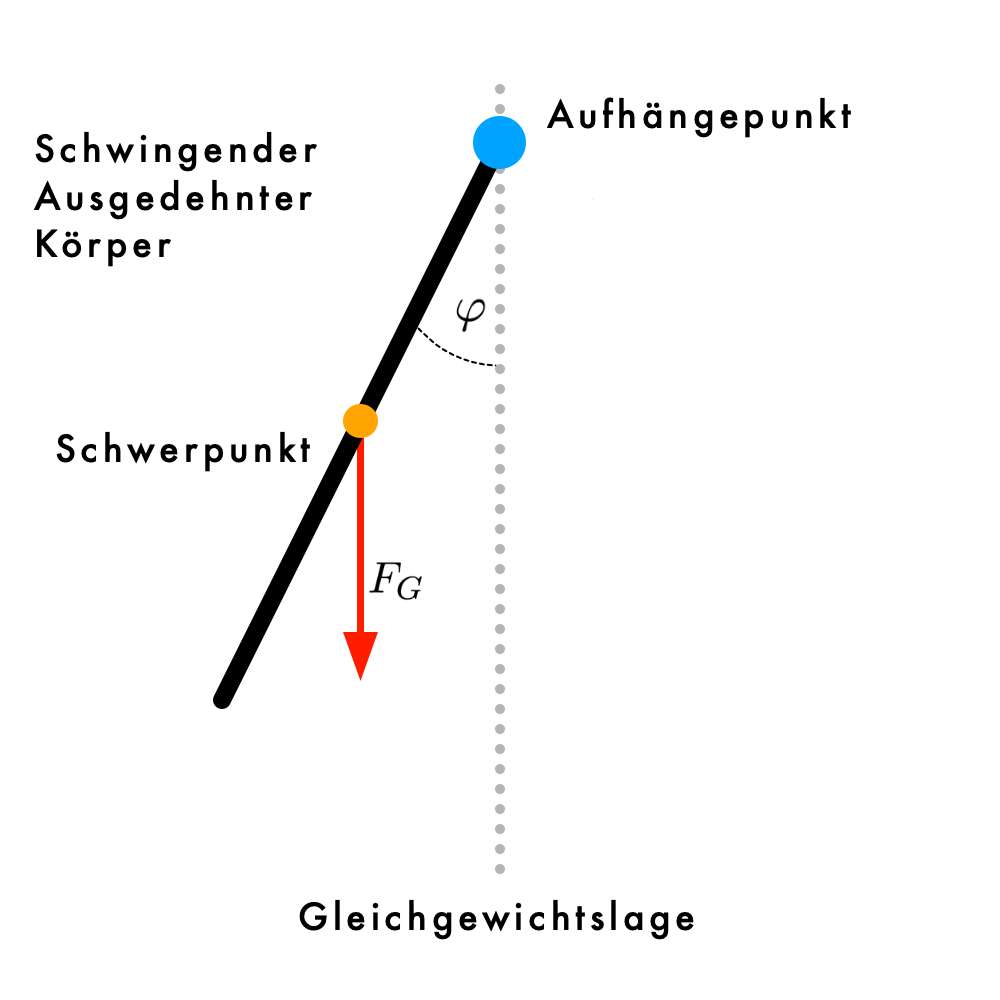
\includegraphics[width=0.4\textwidth]{Spend}
   %\renewcommand\thefigure{B1}
\caption{Versuchsaufbau 1}
\label{JS1}
\end{wrapfigure}

Um diesen Versuchsteil zu durchzuführen wird ein zylindrischer Stab der an einem Stativ gehängt werden kann verwendet. Zusätzlich werden ein Bandmass, Messschieber und eine Stoppuhr für die Messungen benötigt. 



\FloatBarrier
\subsection{Durchführung}

Zuerst wurde die Länge des Stabes mittels Bandmass gemessen. Daraufhin wurde mit dem Messschieber den Durchmesser des Stabes gemessen. Dann wurde der Stab an das Stativ gehängt und per hand zum Pendeln gebracht. Es wurde mit der Stoppuhr 30 mal eine Periode zeitlich gemessen. Danach wurde einmal 30 Perioden gemessen, um zu schauen welches verfahren ein kleineren Fehler hat. Der Fehler war etwas kleiner bei dem einmal messen von 30 Perioden.

\subsubsection{Auswertung}

\begin{table}[ht]
\caption{Bestimmte Werte (Teil 2)}
$$
\begin{array}{lr}
	\toprule 
	\textrm{Stablänge} & l = 96.7(3)\,\textrm{cm} \\
	\textrm{Radius} & r = 0.50(1)\,\textrm{cm} \\
	\textrm{Stablänge bis zum Aufhängepunkt} & a = 95.6(3)\,\textrm{cm}\\
	\textrm{Abstand Aufhängepunkt zu Schwerpunkt} & d = 49.5(5)\,\textrm{cm}\\
	\bottomrule 
\end{array}
$$
\end{table}
Wobei $d$ mit $d = \frac{l}{2} - (l - a)$ berechnet wurde.
Zuerst wird mit den obigen Herleitungen der theoretische Wert bestimmt. Mit $T = 2\pi \sqrt{\frac{I}{dmg}}$, und dem Einsetzen von $I_{\textrm{Stab}}$ bekommt man:
$$T = 2\pi \sqrt{\frac{\frac{1}{4} m r^2 + \frac{1}{3} m l^2}{dmg}} = 2\pi \sqrt{\frac{\frac{1}{4} r^2 + \frac{1}{3} l^2}{dg}}$$

mit $|g|=9.802\dots$\,$\nicefrac{\textrm{m}}{\textrm{s}^2}$\footnote{Dieser Wert wurde in einem anderen Versuch (Einleitungsversuch) bestimmt.} ist der theoretische Wert $T_0 = 1.593(5)$\,s wobei die Unsicherheit $\Delta T = 0.005$\,s mit der Gaußschen Fehlerfortpflanzung gefunden wurde:
$$\Delta T = \sqrt{ \bigp{\pard{T}{r}\Delta r}^2 + \bigp{\pard{T}{l}\Delta l}^2 + \bigp{\pard{T}{d}\Delta d}^2 }$$

Der experimentell bestimmte Mittelwert für 30 einzelne Perioden ist $T_1 = 1.591$\,s mit der Standardabweichung $s_T = 0.05$\,s und der Standardabweichung des Mittelwerts $s_{\bar T} = 0.01$\,s. 

Der exprerimentell bestimmte Wert für eine Messung von 30 Perioden ist $T_2 = 1.594\,$s mit der Unsicherheit von der Gesamtzeit $u_T = \pm0.3$\,s woraus die Unsicherheit $\frac{u_T}{\sqrt{n}} = 0.05$\,s der einzelnen Perioden kommt.

Also sind die drei Werte für die Schwingungsdauer:
$$T_0 = 1.593(5)\,\textrm{s} \qquad T_1 = 1.59(1)\,\textrm{s} \qquad T_2 = 1.59(5)\,\textrm{s}$$

\pagebreak

\section{Teil 2 - Steinersche Satz}

\subsection{Aufbau}

\halftime{5}{5}{Zu diesem Versuch wurde ein Drehpendel verwendet, der aus einer Zusatzmasse, Drehtisch und einer Spiralfeder besteht. Die Zusatzmasse kann in verschiedenen Abständen von dem Mittelpunkt befestigt werden. Für die Messungen wurde eine Stoppuhr und ein Messschieber verwendet.}{
\centering
\fbox{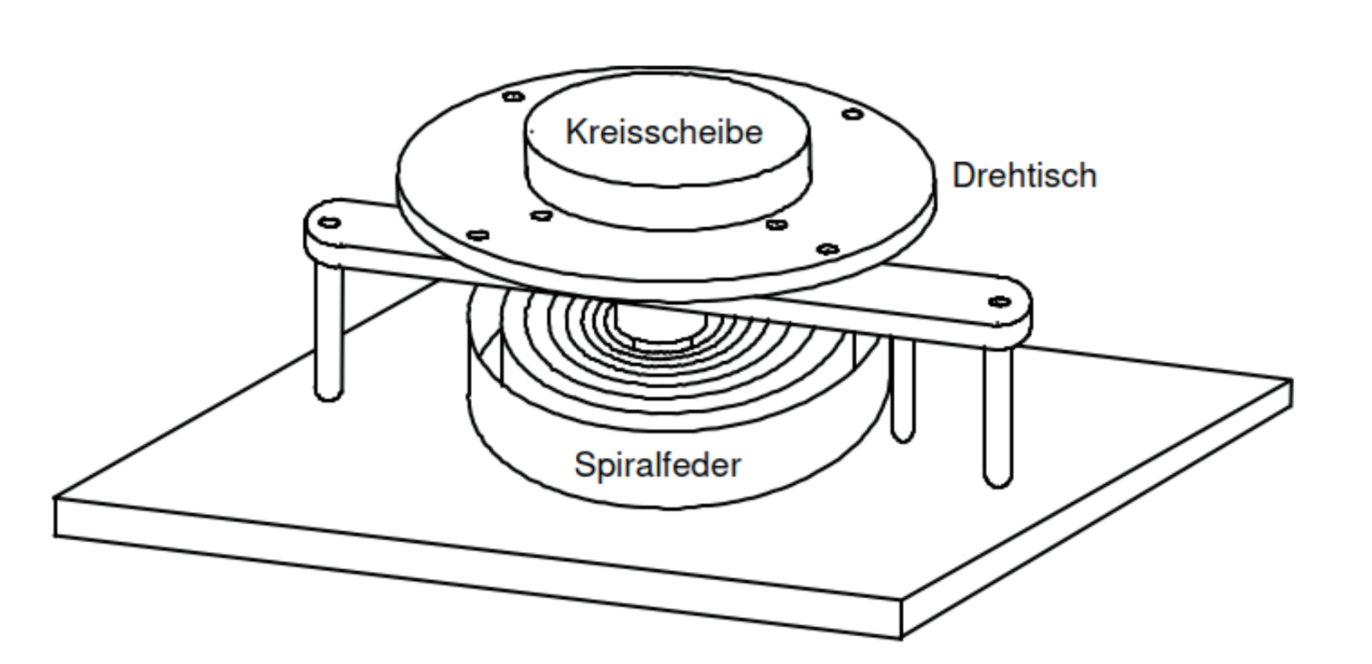
\includegraphics[width=0.7\textwidth]{Drehp}}
   \renewcommand\thefigure{B2}
\caption[Versuchsaufbau 2]{Versuchsaufbau 2 \cite{Anleitung}}
\label{B2}
}

\subsubsection{Durchführung}

Es wurden Breite und Durchmesser der Zusatzmasse mit dem Messschieber gemessen. (Die Masse wurde schon vorher bestimmt und auf das Pendel oben drauf Geschrieben.) Zunächst wurde die Zeit für 30 Perioden ohne Zusatzmasse gemessen. Danach wurde die Masse in den Mittelpunkt gesetzt und  derDrehtisch wurde von Hand soweit aus gelenkt, dass 30 Perioden zeitlich gemessen werden konnten. Dies wurde wiederholt für 10 Perioden. Anschliessend wurde die Masse mit einem Abstand von 15\,mm versetzt und wieder jeweils 30 und 10 Perioden gemessen. Diese Messung wurde wiederholt für vier weitere Abstände. 

\subsection{Auswertung}

\begin{table}[ht]
\caption{Relevante Werte (Teil 2)}
$$
\begin{array}{ll}
	\multicolumn{1}{l}{\textrm{Zu Bestimmende Werte}} \\
	\toprule 
	\textrm{Zusatzmasse} & m = 1.109(5)\,\textrm{kg} \\
	\textrm{Durchmesser} & d = 118.9(1)\,\textrm{mm} \\
	\textrm{Breite} & h = 12.9(1)\,\textrm{mm} \\
	\bottomrule \\
	\multicolumn{2}{l}{\textrm{Bekannte Werte}} \\
	\toprule
	\textrm{Abstände} & a = 15.0\,\textrm{mm}\cite{Anleitung}\\
	\bottomrule 
\end{array}
$$
\end{table}

Der theoretische Wert für das Trägheitsmoment der Drehscheibe ist mit der Formel \ref{pop}:
$$I_{\textrm{Scheibe}} = 0.001960(9)\textrm{kg}\,\textrm{m}^2$$
Die Unsicherheit wurde mit $\Delta I = \frac{I}{2}\sqrt{\bigg(\frac{\Delta m}{m}\bigg)^2 + \bigg(2\frac{\Delta r}{r}\bigg)^2}$ berechnet. 
Um das Trägheitsmoment ohne Zusatzmasse zu berechnen wird mit $\vec M = -D\cdot \varphi$:
$$T = 2\pi \sqrt{\frac{I}{D}}\quad \Rightarrow \quad I = \frac{T^2}{4\pi^2}D$$
Der Satz von Steiner lautet:
$$I_0 = I_a + ma^2$$
Daraus folgt:
$$\frac{T_0^2}{4\pi^2}D = \frac{T_a^2}{4\pi^2}D + ma^2 \quad \Rightarrow \quad T_0^2 = T_a^2 + 4\pi^2 \frac{m}{D}a^2$$
Eine lineare regression wurde in \ref{t17} mit Mathematica durchgeführt. Die Steigung dieser Funktion ist: $4.19(4) + 0.00050(2) x$ 



\section{Diskussion}

\vfill

\begin{thebibliography}{9}
 %\bibitem{Uncertainties}''Correlations between variables are automatically handled, which sets this module apart from many existing error propagation codes.'' - https://pythonhosted.org/uncertainties/
 \bibitem{Anleitung} Physikalisches Institut der Albert-Ludwigs-Universität Freiburg (Hrsg.) (08/2018): Versuchsanleitungen zum Physiklabor für Anfänger*innen, Teil 1, Ferienpraktikum im Sommersemester 2018.
 \end{thebibliography}

\pagebreak

\section{Anhang}

\begin{table}[h]
\caption{Messwerte (Teil 2)}
$$
\begin{array}{cccc}	
	\toprule 
	\textrm{Abstand/mm} & \textrm{10 Perioden/s} & \textrm{30 Perioden/s} & \textrm{Mittelwert/s}\\ 
	\midrule
	\multicolumn{1}{l}{\textrm{Ohne Zusatzmasse}} & 18.1 & 54.6 & 1.82(1)\\
	\phantom{zz.}0 & 20.6 & 60.3 & 2.04(4)\\
	15.0 & 20.8 & 63.0 & 2.09(1)\\
	30.0 & 21.8 & 63.2 & 2.14(5)\\
	45.0 & 22.9 & 68.9 & 2.29(1)\\
	60.0 & 24.9 & 72.0 & 2.45(6)\\
	\bottomrule 
\end{array}
$$
\end{table}

\begin{figure}[h]
\centering
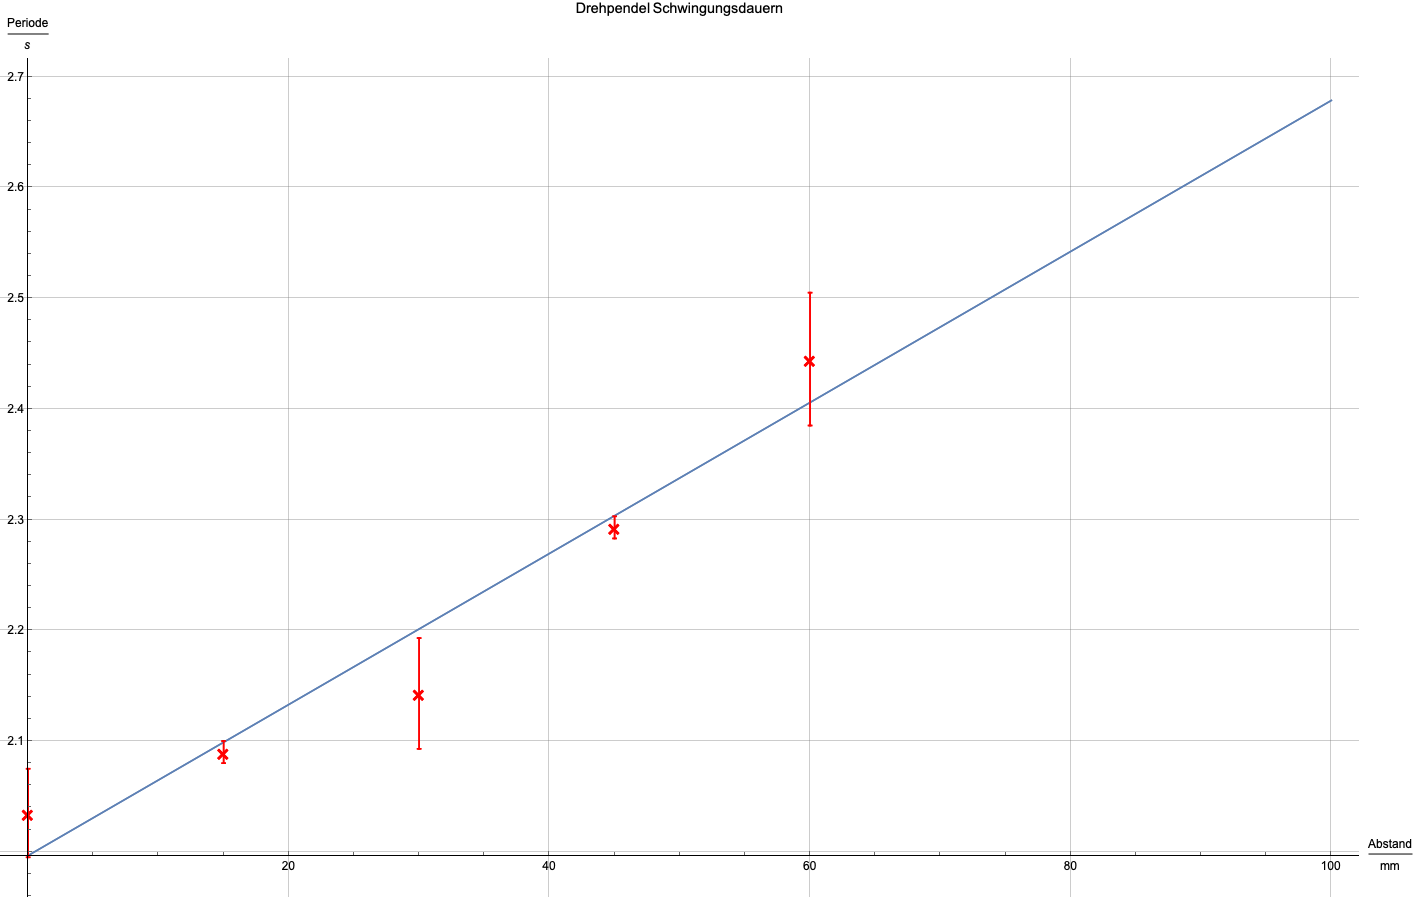
\includegraphics[width=1\textwidth]{trick17}
\renewcommand\thefigure{B3}
\caption{Mittelwerte}
\label{t17}
\end{figure}


\end{document}